\documentclass[../assignment4.tex]{subfiles}
\graphicspath{{\subfix{../figures/assignment4/}}}

\begin{document}
\begin{figure}[h]
    \centering
    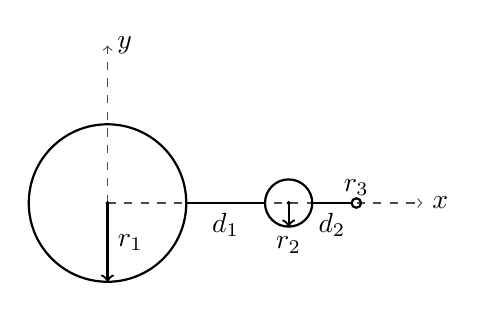
\begin{tikzpicture}
        \draw[->,color=black!70,dashed] (0,0)--(4,0) node[right,black]{$x$};
        \draw[->,color=black!70,dashed] (0,0)--(0,2) node[right,black]{$y$};
        \draw[black,thick] (0,0) circle[radius=1cm] node {};
        \draw[black,thick] (2.3,0) circle[radius=0.3cm] node {};
        \draw[black,thick] (3.16,0) circle[radius=0.06cm] node {};
        \draw[black,thick] (1,0) -- (2,0) node[midway,below] {$d_1$};
        \draw[black,thick] (2.6,0) -- (3.1,0) node[midway,below] {$d_2$};
        \filldraw[black] (0,0) circle (0.5pt) node{};
        \filldraw[black] (2.3,0) circle (0.5pt) node{};
        \draw[->,black,thick] (0,0) -- (0,-1) node[midway,right] {$r_1$};
        \draw[->,black,thick] (2.3,0) -- (2.3,-0.3) node[below] {$r_2$};
        \draw (3.16,0.2) node{$r_3$};
    \end{tikzpicture}
    \caption{The Sun-Earth-Moon system}
    \label{cg4-diagram}
\end{figure}
\end{document}